\documentclass[10pt, conference, compsocconf]{IEEEtran}

% Various packages that might be useful
\usepackage[pdftex]{graphicx}
\usepackage{array}
\usepackage[tight,footnotesize]{subfigure}
\usepackage{url}
\hyphenation{op-tical net-works semi-conduc-tor}
\usepackage{color}

\usepackage{tikz}

\usetikzlibrary{arrows}

\begin{document}

\title{Understanding the Impact of Interconnect Failures on System Operation}

\author{\IEEEauthorblockN{Matt Ezell}
\IEEEauthorblockA{High Performance Computing Operations\\
Oak Ridge National Laboratory\\
Oak Ridge, TN\\
ezellma@ornl.gov}
}

\maketitle

\begin{abstract}

Hardware failures are inevitable on large high performance computing systems.
Faults or performance degradations in the high-speed network can reduce the
entire system's performance. Since the introduction of the Gemini interconnect,
Cray systems have become resilient to many networking faults that were fatal in
their previous generation systems. These new network reliability and resiliency
features have enabled higher uptimes on Cray systems by allowing them to
continue running with reduced network performance. Oak Ridge National
Laboratory has developed a set of user-level diagnostics that stresses the
high-speed network and searches for components that are not performing as
expected. Nearest-neighbor bandwidth tests check every network chip and network
link in the system. Additionally, performance counters stored on the network
ASIC's memory mapped registers (MMRs) are used to better understand the state
of the network. Applications have also been characterized under various
suboptimal network conditions to better understand what impact network problems
have on user codes.

\end{abstract}

\begin{IEEEkeywords}
HPC; Cray; Gemini; Interconnect; HSN; Titan
\end{IEEEkeywords}

\section{Introduction} 

Hardware failures are inevitable on large high performance computing systems.
Problems on a specific compute node can be fatal to an application running on
that node, but these types of faults typically have little to no impact on
other jobs or system services. Faults or performance degradations in the
high-speed network, however, have the potential to reduce the entire system's
performance.

Since the introduction of the Gemini System Interconnect, Cray high performance
computing systems have become resilient to many types of high-speed networking
faults that were fatal in their previous generation systems. Hardware and
software monitoring allow the network to transparently mask out bad lanes
within a link, and to reroute around completely failed links by temporarily
pausing network traffic while installing the new routes. These new network
reliability and resiliency features have enabled higher uptimes on Cray systems
by allowing them to continue running with reduced network performance.

Oak Ridge National Laboratory has developed a set of user-level diagnostics
that stresses the high-speed network and searches for components that are not
performing as expected. Nearest-neighbor bandwidth tests check every network
chip and network link in the system. Unidirectional single-threaded bandwidths
approaching 7 GB/sec have been achieved across healthy links on a quiet system.
Additionally, performance counters stored on the network ASIC's memory mapped
registers (MMRs) are used to get a more full picture of the state of the
network. Applications have also been characterized under various suboptimal
network conditions to better understand what impact network problems have on
user codes.

\section{The Cray Gemini Network}

Cray XE and XK systems are highly scalable supercomputing platforms based on
the Cray Gemini System Interconnect.  Gemini is a fault-tolerant network
configured in a three dimensional torus.

\subsection{Physical Layout}

At the highest level, XE and XK systems are divided up into cabinets.  Cabinets
are arranged ``left to right'' in rows, and larger systems will have multiple
rows.  Cabinets in the same ``left to right'' position in different rows form
columns.  Each cabinet consists of an L1 cabinet controller, a blower fan,
power conversion electronics, and three chassis.  A chassis (also known as a
cage) holds eight modules (also known as blades).  Figure \ref{fig:cab} shows a
cabinet's layout.

Modules contain a network mezzanine that houses two Gemini network chips; each
Gemini is shared between two nodes.  The module printed circuit board layouts
are different between service and compute modules because the service nodes
support PCI Express interface cards.  Furthermore, XE and XK blades differ due
to the absence or presence of a Graphics Processing Unit (GPU).

\begin{figure}
  \centering
  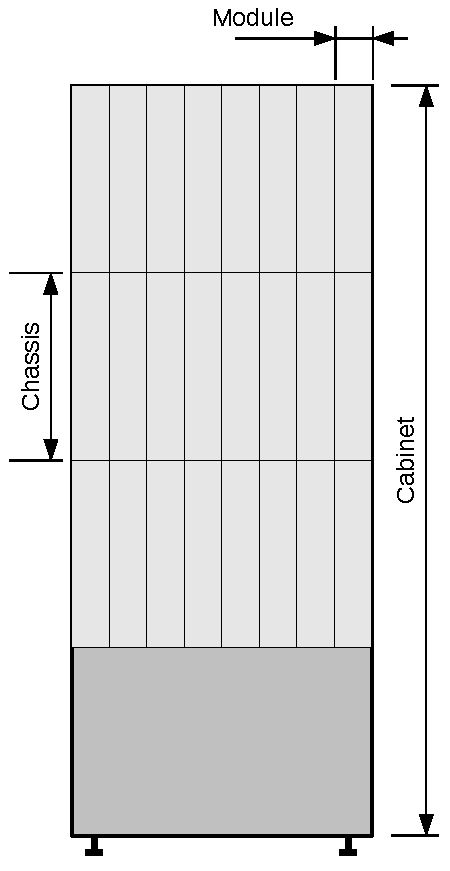
\includegraphics[width=3.0in]{figures/cabinet_diagram.pdf}\\
  \caption{Cabinet Diagram}\label{fig:cab}
\end{figure}

\subsection{3D Torus Topology}

\label{sec:torustopo}
In Gemini's three dimensional torus, each Gemini chip is directly connected to
six of its nearest neighbors: positive and negative X, Y, and Z.  This maps
extremely well to applications that do many nearest-neighbor exchanges, but the
interconnect can be stressed by applications that do all-to-all type
communications.

In general, the X dimension goes along rows, the Y dimension goes along
columns, and the Z dimension goes between the modules in a cabinet.  The
specific cabling rules depend on the size and ``class'' of the system.  For
large systems, X cables connect the 48 Gemini network chips in a cabinet to 48
other Gemini network chips in an X+ cabinet in the same row and 48 other Gemini
network chips in a X- cabinet in the same row.  The length of the X dimension
is equal to the number of columns in a row.  The Y dimension connects the two
Gemini chips that share a mezzanine, and those chips connect to other cabinets
in the same column.  There are 24 Y+ and 24 Y- connections from each cabinet.
The length of the Y dimension is twice the number of rows.  The Z dimension
stays within a cabinet, connecting one Gemini from each module.  There are two
Z-loops per cabinet each with length 24.

Nodes that are close physically are not necessarily close topologically.  Cray
uses a ``folded torus'' to minimize the maximum cable length.  For the X and Y
dimensions, every other cabinet is directly connected together with
``loopback'' cables at the ends to achieve a full torus (see Figure
\ref{fig:cabfold} for an example in the X dimension).  In the Y dimension, the
uppermost chassis connects to the lowermost chassis.

\begin{figure}
  \centering
  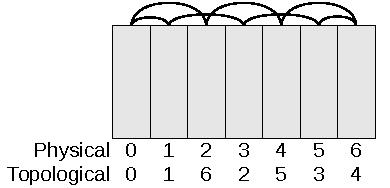
\includegraphics[width=3.0in]{figures/cabinets_folded.pdf}\\
  \caption{Example X Cabinet Connections}\label{fig:cabfold}
\end{figure}

\subsection{The Gemini Network Chip}

Many low-level details about Gemini are available in a paper titled ``The
Gemini System Interconnect'' that appeared in the 2010 IEEE Symposium on High
Performance Interconnects \cite{hoti}.

The Gemini ASIC is a 48-port router than provides two network interface
controllers.  The Gemini router is built using a 6x8 array of identical
``tiles.''  Eight tiles referred to as ``ptiles'' are dedicated to the network
interface controllers, and the remaining 40 ``ntiles'' are dedicated to
external connections.  Figure \ref{fig:tiles} shows the tile assignment; being
able to map link numbers to physical locations and dimensions can help decode
log messages and assist in understanding performance concerns.

\begin{figure}[h]
  \centering
  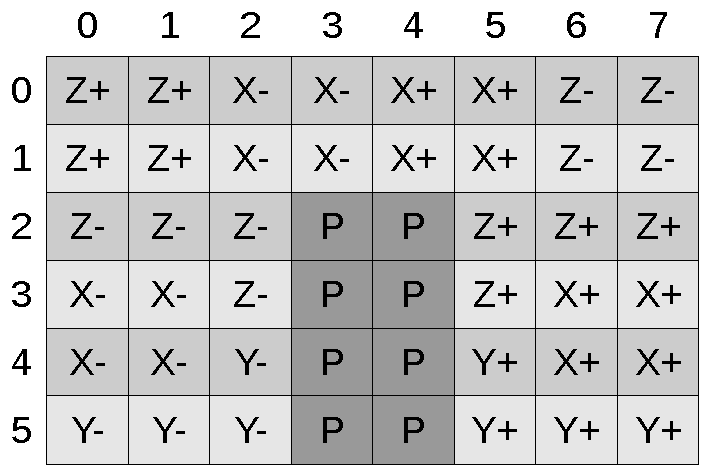
\includegraphics[width=3.0in]{figures/gemini_tiles.pdf}\\
  \caption{Gemini Tile Layout}\label{fig:tiles}
\end{figure}

The Gemini chip also implements hundreds of 64-bit performance counters that
are accessible through memory-mapped registers (MMRs).  The network resiliency
software uses the MMRs to control network performance and identify problems,
but they are also accessible to users (through CrayPat or PAPI).

% This figure belongs further down, but we are defining it here to force placement
\begin{figure*}[ht]
  \begin{verbatim}
130325 15:51:00  c0-0c1s0g0l27     c0-0c1s1g0l17       1 Mode Exchanges                       
130325 15:51:00  c0-0c1s0g0l27     c0-0c1s1g0l17       1 RX lanemask=3                        
130325 15:51:00  c0-0c1s0g0l27       ***ERROR*** Gemini LCB lane(s) reinit failed
130325 15:52:00  c0-0c1s1g0l17     c0-0c1s0g0l27       1 TX lanemask=3                       
  \end{verbatim}
  \caption{Single Lane Degrade Seen in Netwatch File}\label{fig:lanedegrade}
\end{figure*}

\subsection{Network Links}

Each Gemini chip supports two nodes, and those nodes share a topology
coordinate.  Between Gemini chips, there are many ``lanes'' that work in
concert to transfer data.  Three lanes comprise a ``link'' that maps to a
single network tile.  Four links connect in each of the positive and negative
directions in the Y dimension.  For X and Z, there are eight links in each
direction.

The link speed depends on the link type.  Protocol overheads are about 35\% for
large messages.  The expected bandwidths are shown in Table
\ref{tab:linkspeed}.

\begin{table}[h]
  \centering
  \caption{Gemini Link Speeds}
  \label{tab:linkspeed}
  \begin{tabular}{ | c | c | c | c | c | }
    \hline
    Link Type	& Data Rate	& \# Links	& Bitrate	& Data Rate	\\ \hline \hline
    Y-Mezzanine & 6.25 gbps	& 12		& 9.375 GB/s	& \textasciitilde6 GB/s	\\ \hline
    Z-Backplane & 5.0 gbps	& 24		& 15 GB/s	& \textasciitilde9.75 GB/s	\\ \hline
    X,Z Cable	& 3.125 gbps	& 24		& 9.375 GB/s	& \textasciitilde6 GB/s	\\ \hline
    Y Cable	& 3.125 gbps	& 12		& 4.6875 GB/s	& \textasciitilde3 GB/s	\\ \hline
  \end{tabular}
\end{table}

\subsection{Routing and Faults}

The Gemini network uses dimension ordered routing.  In a faultless network,
traffic will first travel along the X dimension until it reaches the
destination node's X coordinate.  The packet will then travel in the Y
dimension to the destination node's Y coordinate.  Finally, it will move in the
Z dimension until it reaches the final destination. 

When faults are present in the network, the routing algorithm must send traffic
in non-optimal ways to ensure that all nodes can communicate.  This will likely
cause some network links to be underutilized while others become
oversubscribed.  Certain failure patterns, such as multiple failures in the
same ``loop'' of the Z dimention, will cause an unrouteable situation.  Recent
improvents to the routing software enabled dimension order retry.  If the
standard X-Y-Z ordering does not work, it will try alternate combinations until
it finds a routeable configuration.

\subsection{Fault Tolerence}

The Gemini network was designed to be tolerant of network faults.  Both
hardware and software support allow the system to withstand many different
types of failures without requiring a system reboot.  When a lane fails, the
network is automatically able to run in a degraded mode.  The lane with an
abnormal number of errors is deactivated and the Gemini balances the traffic
over the other two lanes within the channel.  For a configurable period of
time, the Gemini will attempt to re-initialize the failed lane to restore full
bandwidth.  An example of a degraded lane is shown in Figure
\ref{fig:lanedegrade}. 

% This is where the lane degrade figure *should* go, but we are moving it up so
% it will show up at the top of a page

The lanemask value is a three-bit number corresponding to the three lanes in a
link.  A lanemask of 7 indicates that all lanes are working properly.  A
lanemask of 3, 5, and 6 indicate that a single lane has failed.  A lanemask of
1, 2, or 4 indicates that two lanes have failed.

If an entire link becomes unavailable, the system must take more invasive
action to allow communication to continue.  The Cray Network Link Recovery
Daemon (\emph{nlrd}) on the System Management Workstation (SMW) detects failures and
responds appropriately.  Network traffic is quiesced and new routing tables
(excluding the failed links) are computed and asserted to each Gemini chip.
Then traffic is again allowed to flow using the updated routes.

\subsection{Network Congestion}

Network congestion is a serious problem in any network, especially a 3D torus.
Hot spots in the interconnect can cause variable performance, network timeouts,
or even serious errors.  Not only will the application causing the problem be
affected, but all running processes on the system might be impacted.  Cray
systems employ special hardware and software to avoid congestion.  By reducing
the available injection bandwidth, misbehaving applications are no longer able
to cause congestion.

\subsubsection{Active Throttling}

A network daemon runs on each module controller and regularly samples the MMR
values of the Gemini chips.  When the ratio of network stalls to forwarded
flits (network flow control units) exceeds a configurable value for a
configured period of time, it sends a message to \emph{nlrd} on the SMW indicating
that congestion is occurring.  \emph{nlrd} cooperates with the Application Level
Placement Scheduler (ALPS) to know which applications are running on each node.
\emph{nlrd} sends a message to all the Gemini chips that host the nodes with the
offending application instructing them to throttle.

\subsubsection{Auto-Throttling}

The L0 module controllers must remain in constant contact with \emph{nlrd} on
the SMW for active throttling to work properly.  L0s must assume the worst if
they cannot contact the SMW; after a period of communication failure they will
``auto-throttle'' to protect the rest of the network.  Unfortunately, L0s are
unable to log this fact to the SMW when communication problems are present;
system administrators may be unaware of any issues.

Recently a system at Oak Ridge suffered from auto-throttling due to
communication issues.  Some users were intermittently experiencing job timeouts
without any clear explanation.  Upon investigation, it was found that an entire
cabinet was unreachable from the SMW.  The clip on the Ethernet cable
connecting the cabinet to the master switch was broken and the cable had come
loose.  After reseating the cable and ensuring communication was working
properly, user jobs returned to their normal speed.

\subsubsection{Balanced Injection}

\label{sec:bi}

Certain applications or libraries are known to cause congestion due to their
communication pattern.  Improved performance can be obtained by reducing each
node's injection bandwidth to reduce overall network pressure.  The Gemini
supports the ``balanced injection'' feature to reduce credits and outstanding
request buffers.  Cray's MPICH libraries can automatically enable the balanced
injection mode when performing collectives known to cause issues.
Additionally, users can specify a desire to use balanced injection by setting
the \textbf{APRUN\_BALANCED\_INJECTION} environment variable to a positive
integer less than or equal to 100.

\section{The TopoBW Microbenchmark}

A desire to better understand the state of the high speed network arose during
acceptance testing on Titan.  Several applications were exhibiting extremely
variable behavior, and it was observed that application placement was an
important factor.  Performance improved significantly by packing applications
into submeshes.  Though it is obvious that optimally placed application have
the ability to perform better than poorly placed ones, the degree to which
performance depended on placement seemed excessive to the author.  A benchmark
application was developed to check the health of the high-speed network to
ensure that there were no undiscovered hardware issues.

\subsection{Program Overview}

The TopoBW microbenchmark was designed to test the bandwidth between
nearest-neighbor partners.  When run on an otherwise idle system, nodes can
accurately measure the speed in which they can send and receive messages from
their neighbors.  The basic outline of the application follows:

\begin{itemize}
	\item Determine its topological coordinates and find its topological neighbors
	\item For each dimension and direction, send and receive MPI messages from its neighbors
	\item Aggregate the results and report minimum, average, and maximum bandwidths
\end{itemize}

\subsection{Topology Awareness}

The Cray programming environment makes application geometry as well as physical
and topological coordinates available to userspace applications.  The
\emph{PMI} module provides function calls to determine the number of MPMD
applications launched, number of PEs on a given node, and a mapping of ranks to
nodes.  The \emph{RCA} module provides functions to look up a node's physical
characteristics (such as row, column, cage, slot, and node-number), topological
coordinates, and retrieve the maximum value for each dimension.

The application must discover its six nearest neigbhors.  Two nodes share a
Gemini as well as a topological coordinate;  in the code, these are referred to
as ``partners.''  This sharing will affect how much bandwidth is available to a
given node-pair, so partners must communicate if they are participating in a
transfer.

\subsection{MPI Messaging}

Timed MPI routines are used to exchange messages between nodes.  With a given
amount of data sent and a duration for which the transfer lasted, a transfer
speed can be calculated.  To ensure optimal bandwidth utilization, the
asynchronous send/receive MPI calls are used and message receives are
pre-posted.  Several iterations of transfers are run, each using several
hundred concurrent sends of 4MB each.  The transfer speed is averaged across
the runs.

The application begins running tests by cycling through each of the three
dimensions.  First, the ``even'' nodes send in the positive direction to the
``odd'' nodes;  then, the ``odd'' nodes send in the negative direction to the
``even'' ones.  Next, the ``odd'' nodes send in the positive direction to the
``even'' nodes; then, the ``even'' nodes send in the negative direction to the
``odd'' nodes.  In the case of a dimension with an odd length, the first and
last nodes must then send to each other.  Though this algorithm (shown in
Figure \ref{fig:phases}) has more steps than a more straightforward approach,
it avoids having a Gemini sending and receiving at the same time.

\begin{figure}[h]
  \centering
  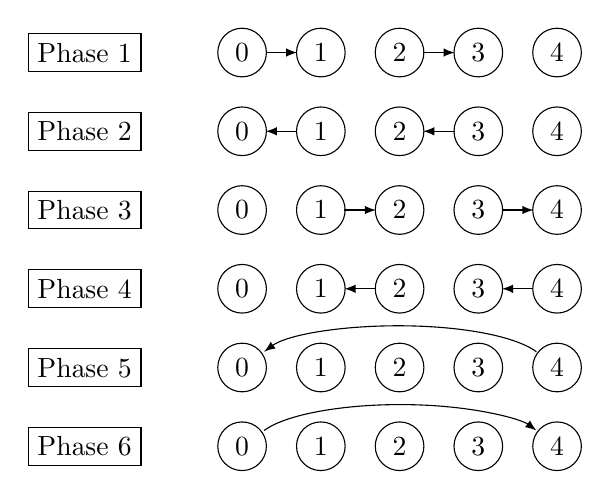
\begin{tikzpicture}
    \def \phase {1}
    \node[draw] at (-1,-\phase) {Phase \phase};
    \node[draw, circle] at (1,-\phase){$0$};
    \node[draw, circle] at (2,-\phase){$1$};
    \node[draw, circle] at (3,-\phase){$2$};
    \node[draw, circle] at (4,-\phase){$3$};
    \node[draw, circle] at (5,-\phase){$4$};
    \draw[->, >=latex] (1.3,-\phase) to (1.7,-\phase);
    \draw[->, >=latex] (3.3,-\phase) to (3.7,-\phase);

    \def \phase {2}
    \node[draw] at (-1,-\phase) {Phase \phase};
    \node[draw, circle] at (1,-\phase){$0$};
    \node[draw, circle] at (2,-\phase){$1$};
    \node[draw, circle] at (3,-\phase){$2$};
    \node[draw, circle] at (4,-\phase){$3$};
    \node[draw, circle] at (5,-\phase){$4$};
    \draw[<-, >=latex] (1.3,-\phase) to (1.7,-\phase);
    \draw[<-, >=latex] (3.3,-\phase) to (3.7,-\phase);

    \def \phase {3}
    \node[draw] at (-1,-\phase) {Phase \phase};
    \node[draw, circle] at (1,-\phase){$0$};
    \node[draw, circle] at (2,-\phase){$1$};
    \node[draw, circle] at (3,-\phase){$2$};
    \node[draw, circle] at (4,-\phase){$3$};
    \node[draw, circle] at (5,-\phase){$4$};
    \draw[->, >=latex] (2.3,-\phase) to (2.7,-\phase);
    \draw[->, >=latex] (4.3,-\phase) to (4.7,-\phase);

    \def \phase {4}
    \node[draw] at (-1,-\phase) {Phase \phase};
    \node[draw, circle] at (1,-\phase){$0$};
    \node[draw, circle] at (2,-\phase){$1$};
    \node[draw, circle] at (3,-\phase){$2$};
    \node[draw, circle] at (4,-\phase){$3$};
    \node[draw, circle] at (5,-\phase){$4$};
    \draw[<-, >=latex] (2.3,-\phase) to (2.7,-\phase);
    \draw[<-, >=latex] (4.3,-\phase) to (4.7,-\phase);

    \def \phase {5}
    \node[draw] at (-1,-\phase) {Phase \phase};
    \node[draw, circle] at (1,-\phase){$0$};
    \node[draw, circle] at (2,-\phase){$1$};
    \node[draw, circle] at (3,-\phase){$2$};
    \node[draw, circle] at (4,-\phase){$3$};
    \node[draw, circle] at (5,-\phase){$4$};
    \draw[<-, >=latex] (1.28,-4.8 ) arc (160:20:1.84 and .5);

    \def \phase {6}
    \node[draw] at (-1,-\phase) {Phase \phase};
    \node[draw, circle] at (1,-\phase){$0$};
    \node[draw, circle] at (2,-\phase){$1$};
    \node[draw, circle] at (3,-\phase){$2$};
    \node[draw, circle] at (4,-\phase){$3$};
    \node[draw, circle] at (5,-\phase){$4$};
    \draw[->, >=latex] (1.28,-5.8 ) arc (160:20:1.84 and .5);
  \end{tikzpicture}
  \caption{TopoBW Phases}\label{fig:phases}
\end{figure}

% This belongs below, but we are definig it here to force placement
\begin{figure*}[ht]
  \begin{verbatim}
c0-0c0s5n1 X+CE c0-0c1s5n1 (nid00011 to nid00053):  5.0454 seconds = 5945.98 MB/sec
c0-0c0s3n2 X+CS c0-0c1s3n2 (nid00024 to nid00038): 10.0846 seconds = 2974.83 MB/sec
c0-0c0s3n3 X+CS c0-0c1s3n3 (nid00025 to nid00039): 10.0851 seconds = 2974.68 MB/sec
c0-0c0s3n0 Y+GS c0-0c0s3n1 (nid00006 to nid00007):  4.4262 seconds = 6777.84 MB/sec
c0-0c0s7n1 Y+ME c0-0c0s7n2 (nid00015 to nid00016):  5.0445 seconds = 5947.03 MB/sec
c0-0c1s0n3 Y+MS c0-0c1s0n0 (nid00033 to nid00062):  5.4767 seconds = 5477.70 MB/sec
c0-0c1s6n3 Z+BE c0-0c1s7n3 (nid00045 to nid00047):  4.4365 seconds = 6762.15 MB/sec
c0-0c1s2n0 Z+BS c0-0c1s3n0 (nid00058 to nid00056):  7.2851 seconds = 4118.02 MB/sec
c0-0c1s2n1 Z+BS c0-0c1s3n1 (nid00059 to nid00057):  7.2847 seconds = 4118.23 MB/sec
c0-0c1s7n0 Z+CS c0-0c1s0n0 (nid00048 to nid00062): 10.5132 seconds = 2853.55 MB/sec
Bandwidth X min: 2974.68 on c0-0c0s3n3 max: 5947.06 on c0-0c1s5n1 avg: 3717.81
Bandwidth Y min: 5437.83 on c0-0c1s3n1 max: 6781.81 on c0-0c1s3n3 avg: 6124.41
Bandwidth Z min: 2667.21 on c0-0c1s0n0 max: 6762.15 on c0-0c1s6n3 avg: 4364.39
  \end{verbatim}
  \caption{TopoBW Sample Output}\label{fig:topobwresults}
\end{figure*}

\subsection{Reporting}

For each node-pair tested the application will emit a line detailing the
conditions present and the performance achieved.  It will list the source and
destination node name and NID as well as the dimension and direction between
the nodes.  An identifier will be present indicating if the ``partner'' node
was also transmitting at the same time or if the link was available exclusively
to that test.  Using the cabling rules described in Section
\ref{sec:torustopo}, the application can identify what type of cable each test
was utilizing.  Since different cable types and dimensions have different
performance characteristics, it is important to understand these details.
Finally, the application will record the duration in which the transfer took
place as well as a calculated data rate in megabytes per second.

At the end of the run, the application will provide a summary of the results.
For each dimension, it will print the minimum, maximum, and average transfer
rates along with the source node on which that rate was achieved.  A subset of
the output is shown in Figure \ref{fig:topobwresults}.

% The reporting figure goes here, but we moved it up to force placement

\subsection{Performance Results}

As expected, performance can vary based on which dimension and cable type are
in use.  The output from Figure \ref{fig:topobwresults} shows that an X cable
sending exclusively can achieve almost 6 GB/sec.  This approaches the bandwidth
limit in the X dimension.  When a similar X link is shared among multiple
send/receive partners the bandwidth halves to less than 3 GB/sec.  The Z
backplane links can achieve over 6.7 GB/s for a single sender, and multiple
senders can achieve over 8.2 GB/s.  In the Y dimension, links are fast between
nodes sharing a Gemini as well as links between two Geminis on the same
Mezzanine.  The bandwidth drops down as it moves to a Y cable.

\subsection{Failures at ORNL}

The TopoBW application can be used to discover slow links within a system.  The
TopoBW output showed a Y- cable that was performing at less-than-expected
speeds.  The system \emph{netwatch} file revealed that the link was suffering
from a lane degrade.

In early January of 2013, the TopoBW application was run on the full
200-cabinet Titan system.  It revealed two Geminis that had consistently poor
results in all dimensions.  The bandwidths never exceeded 4 GB/sec, but the
\emph{netwatch} file did not reveal any problems.

To help narrow down the problem, the affected modules were moved and the system
was rebooted.  TopoBW was again run on the system, and the performance issues
``followed'' the blades to their new locations.  The modules were pulled from
the system and sent to Cray for part failure analysis.  Cray put each module in
a single-slot-tester and examined the signals on the board.  On one module,
they found that it was missing the \emph{L0\_CLKOUT\_3\_HI} signal on the HSN
link between the processor and the Gemini.  Cray replaced the \emph{NeXLev}
mezzanine connector and was able to re-test using TopoBW without failure.

The second module had its \emph{NeXLev} connector replaced but the problem
persisted.  Cray then replaced the \emph{XU7000} Opteron socket and was able to
re-test using TopoBW without failure.

Sometime after the slow modules were removed from Titan, the problematic
acceptance applications were rerun on the system.  Application specialist
reported that the S3D application ran ``significantly faster'' than previously,
but it's not clear how much improvement was due to the removal of the slow
modules.

\subsection{Limitations}

The TopoBW application only tests nearest-neighbor links. Single node injection
bandwidth is less than link bandwidth across the Z backplane; this means that
large performance degradations will be noticed, but small deviations may not be
detected if only a single node-pair is used across that link.

TopoBW is expected to run on the entire system, but this is not a strict
requirement.  Running on a partial system can be useful when there is a desire
to ``spot check'' areas of the torus.  Obviously, this depends on the scheduler
being able to allocate topologically contiguous chunks of the machine.  Another
complication stems from the fact that other applications running on the system
may interfere with TopoBW.  Poorly placed applications or application
performing lots of I/O may send many messages ``through'' TopoBW's node
allocation.  This could result in false positives or variable performance.

%\section{The Latitudes Microbenchmark}

%\subsection{MMR Access}
%ioctl and gpcd


\section{Application Performance Evaluation}

\subsection{S3D: Turbulent Combustion}

Approximately 83\% of U.S. energy comes from the combustion of fossil fuels.
The S3D application simulates turbulent combustion and is being used to enable
the next generation diesels and biofuels to burn more efficiently.  S3D is an
important application for the Oak Ridge National Laboratory Center for
Accelerated Application Readiness (CAAR), and Titan's acceptance plan has
specific performance requirements for S3D. 

Refactoring the S3D code and porting it to the GPU has somewhat moved the major
bottleneck from computation to communication.  Thus, the health and performance
of the Gemini network is essential to the performance observed in S3D.  The
author used S3D as a mechanism to help understand how interconnect problems can
affect application performance.

\subsubsection{Balanced Injection}

The balanced injection feature (see Section \ref{sec:bi}) can be used to
simulate global performance degradation.  S3D was run using 96 nodes on a small
XK7 system using various values for balanced injection.  The results are shown
in Figure \ref{fig:s3dbi}.

\begin{figure}[h]
  \centering
  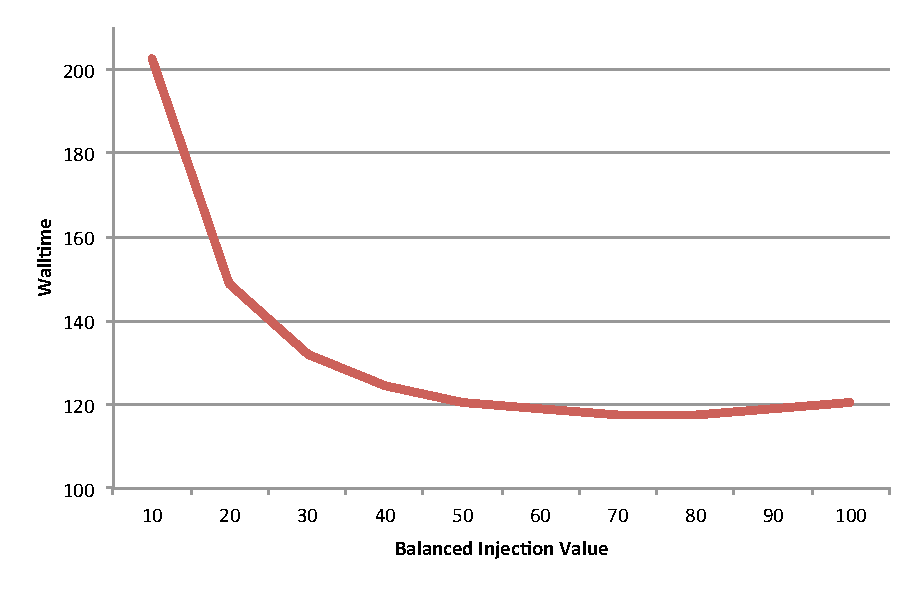
\includegraphics[width=3.4in]{figures/s3d_bisweep.pdf}\\
  \caption{S3D Balanced Injection}\label{fig:s3dbi}
\end{figure}

The shortest walltime is achieved at a balanced injection value of
approximately 70.  This shows that allowing nodes to inject packets into the
network at full speed can cause congestion that reduces performance.
Conversely, limiting injection bandwidth too much will cause performance
degradation.

Since this test was run on a small node count, all communication is relatively
local.  The author expects the results would be more pronounced on larger runs.

\section{Future Work}

Additional work to improve the microbenchmarks is underway.  One possible
improvement would be to exchange the MPI calls for native GNI calls to avoid
overhead.  Native GNI calls also enable more fine-grained control over the
low-level settings associated with each message.  Further research into how the
MMRs are implemented may allow additional information to be extracted from the
Gemini chips.

Currently, the TopoBW application only works on Gemini-based systems.  Future
work will extend the microbenchmark to work on Cray's Aries interconnect.  A
desire also exists to generalize the benchmark so that it can run on commodity
clusters with fat-tree Infiniband interconnects.

Additional combinations of applications and failure scenarios need to be
evaluated to better understand how these failures impact users.  Additional
research is required to develop procedures to manually degrade or disable parts
in ways similar to those observable in production.

\section{Conclusion}

The Gemini interconnect is highly robust and scalable, but it is not immune to
failures and performance problems.  Oak Ridge National Laboratories has
developed an application that can stress the network and find previously
undiscovered performance problems.  It has already identified two faulty
connectors on Titan that caused real performance issues on the system.
Understanding the impacts of network faults on applications helps to prioritize
when issues get fixed, leading to a better overall system.

% use section* for acknowledgement
\section*{Acknowledgment} The author would like to thank several individuals
for providing information and assistance in preparing this paper.  John
Levesque from Cray provided the author with the S3D code and run scripts and
helped resolve some build issues. Bob Alverson from Cray provided some useful
information about Gemini internals, and Kim McMahon from Cray helped track down
a performance anomaly.  Kim Kafka helped coordinate the author's communication
with Cray experts.  Don Maxwell from Oak Ridge National Laboratory reviewed
this paper and provided helpful input.  This research used resources of the Oak
Ridge Leadership Computing Facility at the Oak Ridge National Laboratory, which
is supported by the Office of Science of the U.S.  Department of Energy under
Contract No. DE-AC05-00OR22725. 

% trigger a \newpage just before the given reference number - used to balance
% the columns on the last page adjust value as needed - may need to be
% readjusted if the document is modified later
%\IEEEtriggeratref{8} The "triggered" command can be changed if desired:
%\IEEEtriggercmd{\enlargethispage{-5in}}

% references section

% can use a bibliography generated by BibTeX as a .bbl file
% BibTeX documentation can be easily obtained at:
% http://www.ctan.org/tex-archive/biblio/bibtex/contrib/doc/
% The IEEEtran BibTeX style support page is at:
% http://www.michaelshell.org/tex/ieeetran/bibtex/
%\bibliographystyle{IEEEtran}
% argument is your BibTeX string definitions and bibliography database(s)
%\bibliography{IEEEabrv,../bib/paper}

\bibliographystyle{IEEEtran}
\bibliography{IEEEabrv,hsn}

%\enlargethispage{-2in}

% that's all folks
\end{document}


